\documentclass[11pt]{article}

\usepackage[margin=1in]{geometry}
\usepackage[T1]{fontenc}
\usepackage[utf8]{inputenc}
\usepackage{booktabs}
\usepackage{array}
\usepackage{tabularx}
\usepackage{graphicx}
\usepackage{float}
\usepackage{hyperref}
\usepackage{xcolor}
\usepackage{caption}

\hypersetup{
  colorlinks=true,
  linkcolor=blue,
  citecolor=blue,
  urlcolor=blue
}

\graphicspath{{../results/figures/}{../results_cross_sectional_mvp/figures/}{../results_hardware/figures/}}
\setlength{\parskip}{0.55em}
\setlength{\parindent}{0pt}
\renewcommand{\arraystretch}{1.15}

\newcommand{\project}{QFactor-Penny}
\newcommand{\keyresult}{Cross-sectional-aware feature selection removed the observed QNN constant-score collapse, but QNN rank IC remained negative, precision@3 stayed near random, and no net alpha versus SPY survived transaction costs.}
\newcommand{\smallcode}[1]{{\small\texttt{#1}}}

\title{\textbf{\project: A Reproducible Benchmark of Trainable Quantum Circuits for Cross-Sectional Sector Return Ranking}\\[1.25em]
\large When Small QNNs Fail to Rank Assets Under Walk-Forward Validation}
\author{Tazeem Mahashin\thanks{Rensselaer Polytechnic Institute}}
\date{}

\begin{document}
\maketitle

\begin{abstract}
Quantum machine learning is often proposed for financial prediction, but finance benchmarks are vulnerable to noisy labels, small samples, leakage, and post-hoc overclaiming. We introduce \project, a reproducible PennyLane benchmark for trainable quantum neural networks in cross-sectional sector ETF ranking. The task ranks 11 sector ETFs using non-overlapping five-trading-day rebalance windows, SPY-relative top/bottom labels, expanding walk-forward validation, train-only preprocessing, and transaction-cost-aware portfolio accounting. A 4-qubit PennyLane QNN with angle encoding and one entangling layer is compared against naive momentum, linear models, random forest, RBF-SVM, XGBoost, and a small MLP. The standard QNN did not produce a stable positive ranking signal and exhibited a measurable failure mode: calendar-heavy selected features caused weak cross-sectional sensitivity and constant-score collapse. \keyresult{} The contribution is a leakage-audited QML robustness benchmark and failure-mode analysis, not a quantum-advantage claim.
\end{abstract}

\section{Introduction}

Quantum machine learning is an appealing direction for financial modeling because trainable quantum circuits can represent nonlinear transformations with compact parameterizations \cite{cerezo2021vqa,schuld2021encoding}. Financial ranking tasks, however, are especially vulnerable to small-sample overfitting, target leakage, noisy labels, overlapping forward-return horizons, and post-hoc performance narratives. These concerns are closely related to data-snooping, multiple-testing, and backtest-overfitting risks in empirical finance \cite{white2000reality,bailey2017pbo,harvey2016crosssection}. For quantum finance research to be credible, benchmarks need to report fragility and failure modes with the same care as positive results.

\project{} studies a constrained but realistic task: cross-sectional sector ETF return ranking over non-overlapping five-trading-day rebalance windows. The project does not attempt to forecast exact returns. Instead, each model produces ranking scores for the sector universe, and the benchmark evaluates whether those scores sort the sectors usefully under expanding walk-forward validation.

Small PennyLane QNNs can be implemented cleanly for cross-sectional sector ETF ranking \cite{bergholm2018pennylane}, but under leakage-audited walk-forward validation they did not produce a stable positive ranking signal or post-cost alpha. The main contribution is a reproducible benchmark and failure-mode analysis showing that calendar-heavy feature selection can induce QNN constant-score collapse, and that cross-sectional-aware feature selection can remove the collapse without creating a tradable signal.

The empirical result is negative but informative. The standard QNN run produced constant-score collapse in some rebalance groups and did not generate stable positive rank IC or post-cost alpha. A cross-sectional-aware feature-selection variant removed the constant-score collapse, but the QNN still remained weak as a ranking model. This makes the project a failure-mode benchmark rather than a QNN performance claim.

\keyresult{}

The paper contributes:
\begin{itemize}
  \item A reproducible QML benchmark for finance using non-overlapping five-trading-day sector ETF ranking windows and SPY-relative labels.
  \item A leakage-aware walk-forward evaluation framework with train-only preprocessing, target-window purging, split audits, prediction-shape audits, and deterministic rank handling.
  \item A PennyLane QNN comparison against classical baselines, including linear models, tree models, kernel methods, XGBoost, naive momentum, and a small MLP.
  \item A feature-stability audit showing that calendar-heavy features can break cross-sectional ranking by providing time variation without within-date sector dispersion.
  \item A measured QNN failure mode: constant or near-constant sector scores under standard feature selection.
  \item A diagnostic variant showing that cross-sectional-aware feature selection removes the collapse but does not create stable positive rank signal or post-cost alpha.
\end{itemize}

\section{Data and Prediction Task}

The benchmark uses SPY as the benchmark ticker and excludes SPY from tradable sector portfolios. The tradable universe contains 11 SPDR sector ETFs:
\[
\{\mathrm{XLB}, \mathrm{XLC}, \mathrm{XLE}, \mathrm{XLF}, \mathrm{XLI}, \mathrm{XLK}, \mathrm{XLP}, \mathrm{XLRE}, \mathrm{XLU}, \mathrm{XLV}, \mathrm{XLY}\}.
\]

For each non-overlapping rebalance date, the benchmark computes each sector ETF's next-five-trading-day return and its SPY-relative excess return over the same horizon. The top 3 sectors by forward SPY-relative return receive label 1; the bottom 3 receive label 0; the middle 5 are dropped from classification training. During inference, every model scores all 11 sector ETFs, including the middle sectors.

\begin{table}[H]
\centering
\caption{Task design. SPY is a benchmark/reference only and is never selected in sector portfolios.}
\begin{tabularx}{\textwidth}{@{}lX@{}}
\toprule
\textbf{Design item} & \textbf{Choice} \\
\midrule
Benchmark ticker & SPY \\
Tradable universe & 11 SPDR sector ETFs \\
Horizon & Next 5 trading days \\
Rebalance schedule & Non-overlapping 5-trading-day rebalance dates \\
Training label & SPY-relative top 3 = 1, bottom 3 = 0 \\
Middle sectors & Dropped from classification training, included in inference \\
Inference set & All 11 sector ETFs are scored for every model/date/seed \\
Portfolio & Long equal-weight top 3 sectors \\
Portfolio return & Absolute realized ETF forward return \\
Transaction cost & \texttt{turnover * 0.0005} \\
Alpha definition & \texttt{portfolio\_net\_return - spy\_forward\_return} \\
Tie handling & Model score descending, then ticker as deterministic tie-breaker \\
\bottomrule
\end{tabularx}
\end{table}

\section{Leakage Controls and Walk-Forward Design}

The benchmark uses expanding walk-forward splits. Each split trains on historical rebalance dates, reserves the final training-history slice for validation, and tests on the next month of non-overlapping rebalance dates. Feature selection, imputation, scaling, and model fitting are performed only on training data inside each split.

The split builder applies \smallcode{purge\_trading\_days} before validation and test periods so that five-trading-day forward target windows do not overlap across boundaries. This follows the same spirit as finance ML validation practices that emphasize purging, embargoing, and train-only transformations \cite{lopezdeprado2018afml}. Each run emits \texttt{split\_audit.csv}, which records train, validation, test, purge, and forward-window boundary dates. This audit is central to the paper because it makes leakage controls visible rather than implicit.

\section{Models}

The QNN uses PennyLane's analytic simulator for training. The required MVP architecture maps 4 selected and scaled features to 4 qubits using angle encoding, applies one \smallcode{StronglyEntanglingLayers} layer, and returns a scalar expectation value used as the ranking score. The QNN has 13 trainable parameters in the current implementation.

Classical baselines are intentionally lightweight but nontrivial: naive momentum rank, logistic regression, ridge linear classifier, random forest, RBF SVM, a small one-hidden-layer MLP, and optional XGBoost when installed. The goal is not to exhaust every classical model family. The goal is to prevent the QNN from being compared only to weak straw baselines.

\section{Metrics and Portfolio Accounting}

The benchmark reports both machine-learning and portfolio-style metrics. Ranking quality is summarized using rank IC and precision@3. Classification behavior is summarized using ROC-AUC, balanced accuracy, and F1 where defined. Metrics that are undefined due to constant scores, one-class labels, tiny samples, or zero volatility are reported as \texttt{NaN} with warnings instead of crashing or silently disappearing.

Portfolio evaluation ranks sectors by model score at each rebalance date and selects the top 3 sectors as an equal-weight long portfolio. Gross and net returns use absolute realized ETF returns, not SPY-relative target returns:
\[
\mathrm{turnover}=0.5 \sum_i |w_{i,t} - w_{i,t-1}|,
\]
\[
\mathrm{transaction\ cost}=\mathrm{turnover} \times 0.0005,
\]
\[
\mathrm{net\ return}=\mathrm{gross\ return} - \mathrm{transaction\ cost},
\]
\[
\alpha_{\mathrm{SPY}}=\mathrm{net\ return}-\mathrm{SPY\ forward\ return}.
\]

\section{Results}

Return and alpha values are mean five-trading-day rebalance-period values, not annualized returns.

\subsection{Standard Feature Selection}

In the standard MVP run, train-only mutual-information feature selection selected several calendar-heavy features, including \texttt{month\_cos}, \texttt{weekday\_cos}, and \texttt{month\_sin}. These features varied over time but had zero within-date cross-sectional dispersion across ETFs. That makes them weak inputs for a task that requires ranking sectors against one another on the same rebalance date.

The QNN standard run produced 4 constant-score date groups and 1 row with undefined QNN metrics. Its mean rank IC was -0.0735, precision@3 was 0.2292, and alpha versus SPY after transaction costs was -0.0004.

\subsection{Cross-Sectional-Aware Feature Selection}

The cross-sectional-aware variant filters low within-date dispersion features using only the training slice. This variant is a diagnostic experiment, not post-hoc performance tuning. It tests whether the measured collapse is associated with feature geometry rather than QNN optimization alone.

The variant removed calendar-heavy selected features from the learned-model selected feature set and reduced QNN constant-score groups from 4 to 0. However, the ranking result remained weak: QNN rank IC stayed negative at -0.0494, precision@3 was 0.2708, and alpha versus SPY after costs worsened slightly to -0.0006.

Because the task selects 3 sectors out of 11 and there are 3 true positive sectors, random precision@3 is approximately \(3/11=0.2727\). The cross-sectional-aware QNN precision@3 of 0.2708 is therefore near random.

\begin{table}[H]
\centering
\caption{Standard vs. cross-sectional-aware QNN comparison. Values are from the clean MVP comparison artifacts.}
\begin{tabular}{@{}lrr@{}}
\toprule
\textbf{QNN metric} & \textbf{Standard} & \textbf{Cross-sectional-aware} \\
\midrule
Constant-score groups & 4 & 0 \\
Calendar-heavy selected feature share & 40\% & 0\% \\
Rank IC & -0.0735 & -0.0494 \\
Precision@3 & 0.2292 & 0.2708 \\
Alpha vs. SPY after costs & -0.0004 & -0.0006 \\
Turnover & 0.5521 & 0.6562 \\
\bottomrule
\end{tabular}
\end{table}

\keyresult{}

\subsection{Classical Baseline Context}

The classical baselines also showed unstable behavior in the short MVP comparison. This matters: the negative QNN result is not merely ``classical models win.'' The broader result is that this small, noisy financial ranking task is difficult, and robust reporting should emphasize instability, turnover, and path dependence.

\begin{table}[H]
\centering
\scriptsize
\caption{Model comparison table. Metrics are means from the current standard and cross-sectional-aware MVP comparison.}
\begin{tabular}{@{}llrrrr@{}}
\toprule
\textbf{Model} & \textbf{Feature selection} & \textbf{Rank IC} & \textbf{Precision@3} & \textbf{Alpha vs. SPY} & \textbf{Turnover} \\
\midrule
Logistic regression & Standard & -0.0369 & 0.2292 & -0.0010 & 0.7188 \\
Naive momentum & Standard & -0.0540 & 0.2917 & -0.0023 & 0.3021 \\
PennyLane QNN & Standard & -0.0735 & 0.2292 & -0.0004 & 0.5521 \\
Random forest & Standard & -0.1350 & 0.2292 & -0.0038 & 0.6771 \\
RBF SVM & Standard & 0.0551 & 0.3542 & 0.0004 & 0.6354 \\
Ridge linear & Standard & -0.0403 & 0.2292 & -0.0010 & 0.7188 \\
Small MLP & Standard & -0.0614 & 0.2083 & -0.0023 & 0.7604 \\
XGBoost & Standard & -0.1564 & 0.2083 & -0.0044 & 0.6979 \\
Logistic regression & Cross-sectional-aware & 0.0682 & 0.2292 & -0.0004 & 0.7188 \\
Naive momentum & Cross-sectional-aware & -0.0540 & 0.2917 & -0.0023 & 0.3021 \\
PennyLane QNN & Cross-sectional-aware & -0.0494 & 0.2708 & -0.0006 & 0.6562 \\
Random forest & Cross-sectional-aware & -0.0386 & 0.2917 & -0.0020 & 0.7188 \\
RBF SVM & Cross-sectional-aware & 0.0653 & 0.2917 & -0.0001 & 0.6771 \\
Ridge linear & Cross-sectional-aware & 0.0710 & 0.2500 & 0.0003 & 0.6771 \\
Small MLP & Cross-sectional-aware & -0.0869 & 0.2708 & -0.0016 & 0.5521 \\
XGBoost & Cross-sectional-aware & -0.0175 & 0.3333 & 0.0004 & 0.7812 \\
\bottomrule
\end{tabular}
\end{table}

\begin{figure}[H]
\centering

\includegraphics[width=0.92\textwidth]{model_rank_ic.png}
\caption{Mean model rank IC in the standard MVP run. Positive bars should not be interpreted as statistically significant outperformance; the MVP uses only 4 splits and one seed.}
\end{figure}

\begin{figure}[H]
\centering

\includegraphics[width=0.92\textwidth]{turnover_vs_return.png}
\caption{Turnover versus mean net return in the standard MVP run. High turnover is a practical limitation when interpreting any apparent return.}
\end{figure}

\subsection{Shot Sensitivity}

The QNN is trained analytically and then evaluated on a small fixed subset with 1024-shot simulator sampling. This is an inference-only simulation diagnostic, not real-hardware validation. It does not retrain the QNN with shots.

Under standard feature selection, later splits showed weak or negative analytic-vs-shot score correlation and high ranking flip rates, especially around the constant-score failure. Under cross-sectional-aware feature selection, shot-score correlations were high in the MVP run, but this did not translate into a stable positive ranking signal.

\begin{table}[H]
\centering
\scriptsize
\caption{QNN shot sensitivity. Shot sensitivity is inference-only simulator sampling after analytic training.}
\begin{tabular}{@{}llrrr@{}}
\toprule
\textbf{Variant} & \textbf{Split} & \textbf{Shot score corr.} & \textbf{Mean abs. diff.} & \textbf{Ranking flip rate} \\
\midrule
Standard & split\_00\_2018-12 & 0.9764 & 0.0197 & 0.0000 \\
Standard & split\_01\_2019-01 & 0.8979 & 0.0268 & 0.1481 \\
Standard & split\_02\_2019-02 & -0.4807 & 0.0259 & 0.7143 \\
Standard & split\_03\_2019-03 & -0.6488 & 0.0202 & 0.7692 \\
Cross-sectional-aware & split\_00\_2018-12 & 0.9950 & 0.0219 & 0.0385 \\
Cross-sectional-aware & split\_01\_2019-01 & 0.9969 & 0.0232 & 0.0357 \\
Cross-sectional-aware & split\_02\_2019-02 & 0.9941 & 0.0307 & 0.0000 \\
Cross-sectional-aware & split\_03\_2019-03 & 0.9932 & 0.0203 & 0.1071 \\
\bottomrule
\end{tabular}
\end{table}

\begin{figure}[H]
\centering

\includegraphics[width=0.78\textwidth]{qnn_shot_sensitivity.png}
\caption{QNN 1024-shot sensitivity diagnostic for the standard MVP run only. The plot is simulator-based, not real-hardware validation; cross-sectional-aware shot-sensitivity values are reported separately in Table 4.}
\end{figure}

\section{Failure-Mode Analysis}

The paper's central failure mode is QNN constant-score collapse: the trained circuit emits identical or nearly identical scores for all sector ETFs on a rebalance date. This is damaging for cross-sectional ranking because it destroys sector ordering and can make ROC-AUC, rank IC, balanced accuracy, or F1 undefined.

Feature-stability analysis suggests one mechanism. Standard feature selection sometimes selected calendar-heavy features with time-series variation but no within-date cross-sectional dispersion. A feature such as \texttt{month\_cos} can describe the date, but all sector ETFs on that date receive the same value. If a model leans on these inputs, it may learn date-level context without learning sector-level differences.

The cross-sectional-aware diagnostic supports this interpretation: removing low-dispersion features eliminated the observed QNN collapse. But the diagnostic also shows the limits of the fix. Removing collapse is not the same as finding a robust ranking signal. The QNN still had negative rank IC, near-random precision@3, and negative post-cost alpha versus SPY.

\section{Reproducibility and Artifacts}

\project{} is designed to make experiment state auditable. Each benchmark run writes raw results, aggregate summaries, and diagnostic files.

\textbf{Code and artifact availability.} Code and artifacts are available in the accompanying GitHub repository. The repository includes configuration files for the MVP and cross-sectional-aware MVP runs, \texttt{run\_manifest.json} files with config/data hashes and dependency versions, audit CSVs for splits, predictions, model run status, portfolio selection, feature stability, and QNN failures, generated result summaries, figures, and pytest coverage for leakage controls, portfolio accounting, artifact cleanliness, and paper consistency.

\begin{table}[H]
\centering
\small
\caption{Reproducibility artifacts.}
\begin{tabularx}{\textwidth}{@{}lX@{}}
\toprule
\textbf{Artifact} & \textbf{Purpose} \\
\midrule
\texttt{run\_manifest.json} & Records config hash, dataset hash, dependency versions, seeds, runtime, and output directory. \\
\texttt{split\_audit.csv} & Records train/validation/test dates, purge gaps, and target-window boundaries. \\
\texttt{prediction\_audit.csv} & Confirms every model/date/seed scores all 11 sector ETFs and includes middle-sector inference rows. \\
\texttt{model\_run\_status.csv} & Records success, skip, failure, constant-score dates, NaN scores, and diagnostics availability. \\
\texttt{feature\_stability\_summary.csv} & Reports selected-feature dispersion and calendar-heavy flags. \\
\texttt{qnn\_failure\_audit.csv} & Summarizes QNN constant-score groups, undefined metrics, and selected features. \\
\texttt{quantum\_diagnostics.csv} & Records qubits, layers, parameter count, train/inference time, and shot-sensitivity diagnostics. \\
\texttt{experimental\_variant\_comparison.csv} & Compares standard and cross-sectional-aware feature-selection variants. \\
\texttt{results\_hardware/} & Contains optional frozen-QNN IBM hardware audit CSVs, manifest, summary, and diagnostic figure. \\
\bottomrule
\end{tabularx}
\end{table}

\section{Limitations}

This benchmark is not a trading system and is not investment advice. The current MVP summaries use only 4 walk-forward splits and one seed (42) for fast iteration. The tradable universe is small: 11 sector ETFs. Financial labels are noisy, sector returns are path dependent, and five-trading-day horizons can be unstable. The main benchmark trains the QNN on an analytic simulator, and the 1024-shot experiment is inference-only simulator sampling, not real-hardware validation. The IBM hardware appendix is also inference-only: it runs a small frozen-QNN subset on hardware as a systems robustness audit, not as real-hardware validation of a finance signal. The reported cross-sectional-aware variant is diagnostic, not an optimized production feature pipeline. These constraints are especially important given the known risk of false discoveries and overfit backtests in empirical asset-pricing research \cite{white2000reality,bailey2017pbo,harvey2016crosssection}.

The paper makes no statistical-significance claim, no quantum-advantage claim, and no trading-edge claim. Most importantly, a cleaner diagnostic result should not be overread. The cross-sectional-aware QNN removed constant-score collapse, but it did not create stable positive rank IC or post-cost alpha.

\section{Future Work}

Future work should run the full benchmark across more splits and seeds, expand robustness checks, and report confidence intervals for ranking and portfolio metrics. A larger universe could test whether QNN fragility changes with a broader cross-section, though this would also increase the need for careful multiple-testing controls. Additional QNN variants should be introduced only as pre-registered experimental variants, not as post-hoc tuning to make results look better. A future hardware pass could repeat the exact frozen-QNN audit with a rotated token, higher shot budget, and pre-specified settings, but it should remain a robustness diagnostic unless substantially stronger evidence exists.

\section{Conclusion}

\project{} demonstrates that small PennyLane QNNs can be evaluated rigorously in a financial ranking setting, but the tested QNN did not produce stable positive ranking behavior. The most informative result was a failure mode: standard feature selection sometimes chose calendar-heavy inputs with weak cross-sectional dispersion, leading to QNN constant-score collapse. \keyresult{} These results do not support a quantum-advantage or trading-edge claim. Instead, they support the value of leakage-aware QML benchmarks that expose model fragility before making performance claims.

\appendix
\section{IBM Quantum Hardware Robustness Audit}

After the simulator benchmark, a small frozen-QNN subset was executed on RPI's IBM Quantum System One backend \texttt{ibm\_rensselaer} through the \texttt{General-dedicated} instance. This appendix is a hardware robustness audit, not a new model comparison: the QNN was not retrained on hardware, the benchmark conclusions were not changed, and the run does not validate a finance signal on real hardware.

\begin{table}[H]
\centering
\caption{Inference-only IBM hardware robustness audit for a frozen QNN subset.}
\begin{tabular}{@{}lr@{}}
\toprule
\textbf{Hardware diagnostic} & \textbf{Result} \\
\midrule
Backend & \texttt{ibm\_rensselaer} \\
Backend size & 127 qubits \\
Instance & \texttt{General-dedicated} \\
Samples & 11 frozen QNN inference samples \\
Shots & 100 \\
Optimization / resilience & level 0 / level 0 \\
Mean depth & 8.0000 $\rightarrow$ 26.6364 \\
Mean two-qubit gates & 4.0000 $\rightarrow$ 8.9091 \\
Mean SWAP count & 0.0000 \\
Analytic vs hardware score correlation & -0.0901 \\
Mean absolute score difference & 0.3857 \\
Pairwise ranking flip rate & 0.4630 \\
Top-3 overlap & 0.3333 \\
\bottomrule
\end{tabular}
\end{table}

The analytic top 3 was \texttt{XLP, XLV, XLC}; the hardware top 3 was \texttt{XLK, XLU, XLP}. The mismatch is consistent with a robustness reading: finite-shot hardware execution produced score drift and ranking instability relative to analytic simulation. It should not be interpreted as outperformance, tradable alpha, or quantum advantage.

A first batched optimization-level-1 Estimator attempt failed with IBM HAL error \texttt{9604} (\texttt{Failed to set configuration on HAL components}). The conservative optimization-level-0 execution succeeded and is treated as the canonical v1 hardware artifact. The failure is documented because runtime/HAL behavior is part of the simulator-to-hardware gap this project is meant to expose.

\begin{figure}[H]
\centering
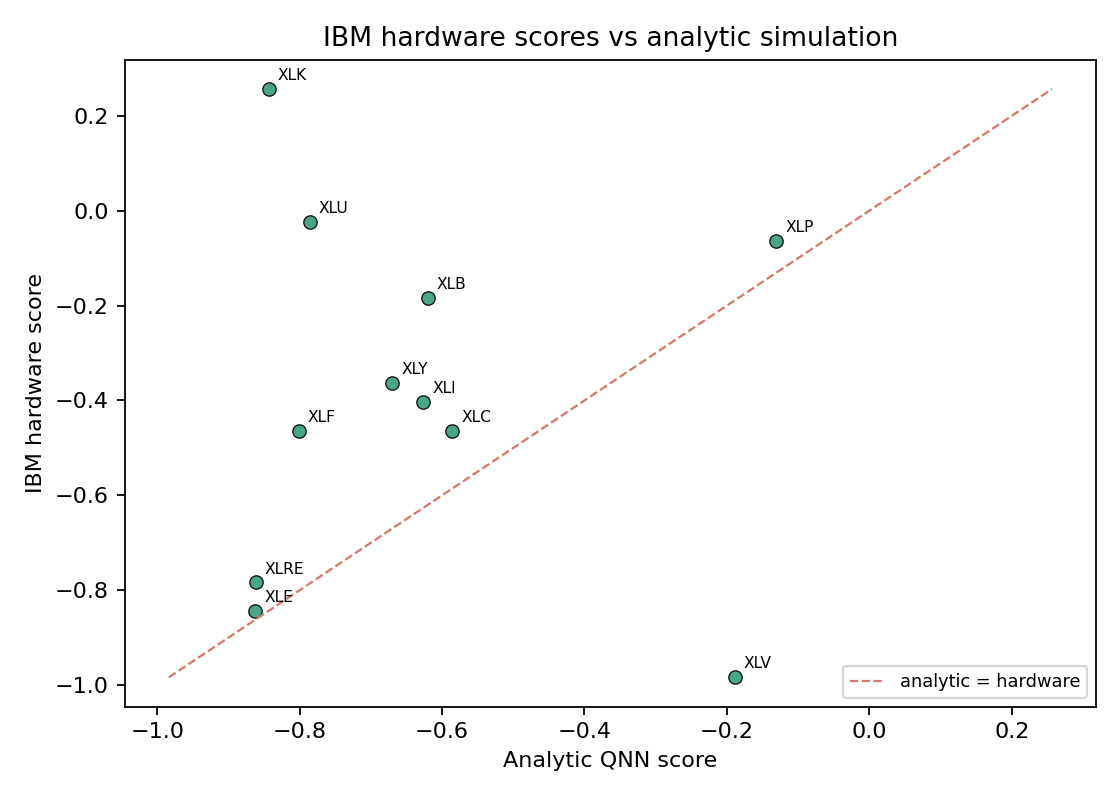
\includegraphics[width=0.78\textwidth]{hardware_score_scatter.png}
\caption{IBM hardware scores versus analytic simulation for the frozen 11-sample QNN subset. This is a hardware diagnostic figure, not evidence of real-hardware validated finance signal.}
\end{figure}

\bibliographystyle{plain}
\bibliography{references}

\end{document}
